\documentclass{beamer}

%% Pacotes
\usepackage[utf8]{inputenc}              %%Formatação de acentos
\usepackage{xcolor}                      %%Definição de cores
\usepackage[framemethod=tikz]{mdframed} %%Estilização dos slides
\usepackage{tcolorbox}                   %%Mudar ambientes de blocos

%\tcbset{colback=red!5!white,
%colframe=red!75!black,fonttitle=\bfseries} %% Borda das caixas

\usepackage[activate={true,nocompatibility},final,tracking=true,kerning=true,spacing=true,factor=1100,stretch=10,shrink=10,expansion]{microtype}
%% Melhorar caligrafia

\SetTracking{encoding={*}, shape=sc}{0} %Caligrafia de small capitals (smallcaps)


\usepackage{pifont} %Dingbats (simbolos do itemize)
\usepackage[alf]{abntex2cite}


%%%%%% NÃO FUNCIONA PRA CLASSE BEAMER %%%%% ~~~
% \renewcommand\labelitemi{\ding{166}} %definindo o símbolo itemize
% padrão a ser utilizado
% \renewcommand{\item}{\ding{166}}
%\newcommand{\itemm}{\ding{\166}}
% \renewcommand\labelitemi{\ding{52}}
%%%%%%%%%%%%%%%%%%%%%%%%%%%%%%%%%%% ~~~

%% Plano de Fundo (corpo)
\usebackgroundtemplate{
  
\includegraphics[width=\paperwidth,
  height=\paperheight]{background.jpg}
}

%% Tema da apresentação
\usetheme{Warsaw}
\usecolortheme{lily}
\usefonttheme{serif}


\mode<presentation>


\title[Gases Especiais]{\Huge{Gases Especiais}}

\author[Guilherme Rosa]{Guilherme Ricardo Dos Reis Rosa \\
  \text{\scriptsize{guilhermericardo8@usp.br}}}

\date[EEL-USP]{\scriptsize{Mini-curso de \LaTeX} \\ Universidade de São Paulo - LabEEL}



%%%%%% ~~~~~~~~~ %%%%%%%%

%%%%%%%%%%% Começo do Corpo do Documento %%%%%%%%%%%%%%%%

%%%%%% ~~~~~~~~~ %%%%%%%%

%%%%CAPA USP%%%%%%

\begin{document}

%% Imagem de fundo para a apresentação,
{\usebackgroundtemplate{
\includegraphics[width=\paperwidth]{logousp.jpg}}

%% Alterar o diretório ''../Imagens/TP.jpg'' para mudar de imagem


%%%%%% Primeira slide, utilizando as variáveis author, date etc.
  \begin{frame}
    \titlepage
  \end{frame}
}


\begin{frame}
  \frametitle{Introdução}

  \begin{enumerate}
  \item<1->[{\textcolor{yellow!90!black}{\ding{254}}}]{O que são ?}
  \item<4->[\ding{58}]{Normas de segurança}
  \item<2->[{\textcolor{red}{\ding{96}}}]{Tipos de Gases}
  \item<3->[{\textcolor{green}{\ding{69}}}]{Aplicações}
  \end{enumerate}

\end{frame}



\begin{frame}

  \section{O que são}
  \frametitle{
    {\textcolor{yellow!70!black}{ {\LARGE \ding{254}}} %Símbolo sol aumentado
      \textcolor{white!100!black}{O que são?}}} %
  \pause
  \begin{tcolorbox}[colback=blue!5!white, colframe=green!65!white,
    title={\sc{\bf{Definição}}}]
    Os \alert{gases especiais} incluem: gases raros, gases da mais alta pureza (cerca de (99,995\% e superior) e misturas de elevada precisão. Muitas indústrias voltadas para as áreas de Analítica e setores petroquímicos utilizam a tempos os gases especiais pelo seu alto nível de pureza, que serve para ajudar a melhorar os processos, otimizar o desempenho e reduzir custos.
  \end{tcolorbox}

\end{frame}

\begin{frame}
	\frametitle{
		{\textcolor{yellow!70!black}{ {\LARGE \ding{254}}} %Símbolo sol aumentado
			\textcolor{white!100!black}{O que são?}}} %
	\begin{tcolorbox}[colback=red!5!white,colframe=red!70!white,title=Citação]
		\begin{itemize}

			\item \cite{kerry2007industrial}
			\bibliography{cite}


		\end{itemize}
	\end{tcolorbox}
\end{frame}

\begin{frame}
	\frametitle{{\textcolor{yellow!70!black}{ {\LARGE \ding{254}}} %Símbolo sol aumentado
			\textcolor{white!100!black}{Imagem}}} %
		\begin{tcolorbox}[colback=blue!5!white,colframe=purple!30!white,title=Imagem]
			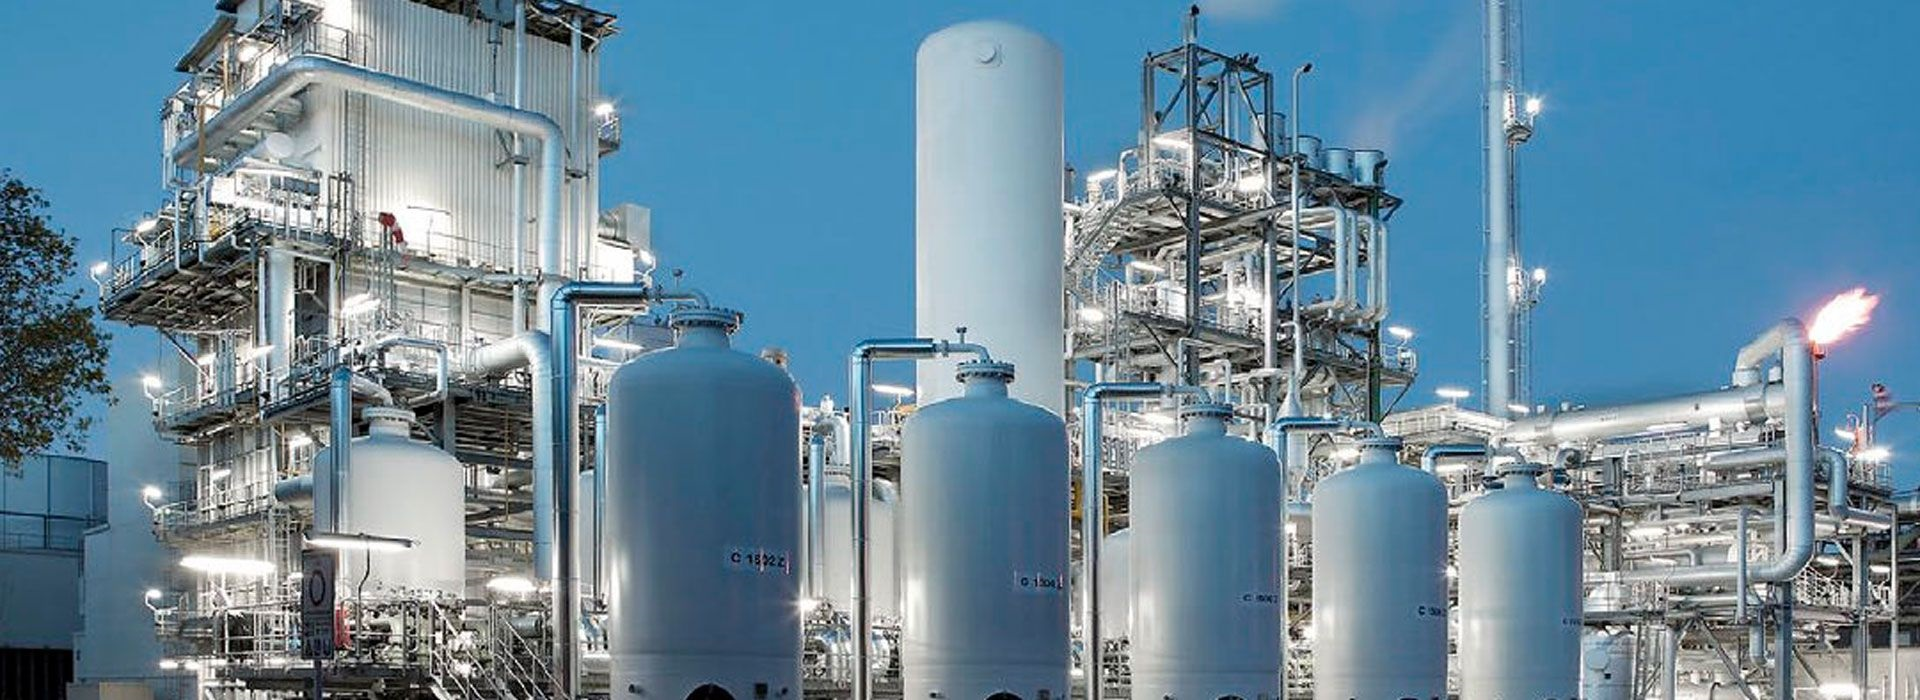
\includegraphics[width=0.5 \paperwidth, height=0.5 \paperheight]{gas}
		\end{tcolorbox}
\end{frame}


\end{document}


%%% Local Variables:
%%% mode: latex
%%% TeX-master: t
%%% End:
